\begin{figure}
    \begin{minipage}[c]{0.67\textwidth}
        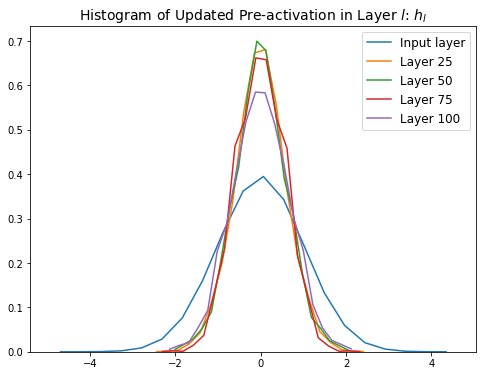
\includegraphics[width=\textwidth]{NodeHistogram}
    \end{minipage}\hfill
    \begin{minipage}[c]{0.3\textwidth}
        \caption{To show that node vanishing is not arise from gradients exploding or vanishing, we plot histograms of hidden nodes of the updated network in figure \ref{fig:sec5_sim2}. We can observe that the scales of hidden nodes are neither vanishing nor exploding.}
        \label{fig:sec6_sim1}
    \end{minipage}
\end{figure}